\documentclass[noinstructornotes]{ximera}
%handout:  for handout version with no solutions or instructor notes
%handout,instructornotes:  for instructor version with just problems and notes, no solutions
%noinstructornotes:  shows only problem and solutions

%% handout
%% space
%% newpage
%% numbers
%% nooutcomes

%I added the commands here so that I would't have to keep looking them up
%\newcommand{\RR}{\mathbb R}
%\renewcommand{\d}{\,d}
%\newcommand{\dd}[2][]{\frac{d #1}{d #2}}
%\renewcommand{\l}{\ell}
%\newcommand{\ddx}{\frac{d}{dx}}
%\everymath{\displaystyle}
%\newcommand{\dfn}{\textbf}
%\newcommand{\eval}[1]{\bigg[ #1 \bigg]}

%\begin{image}
%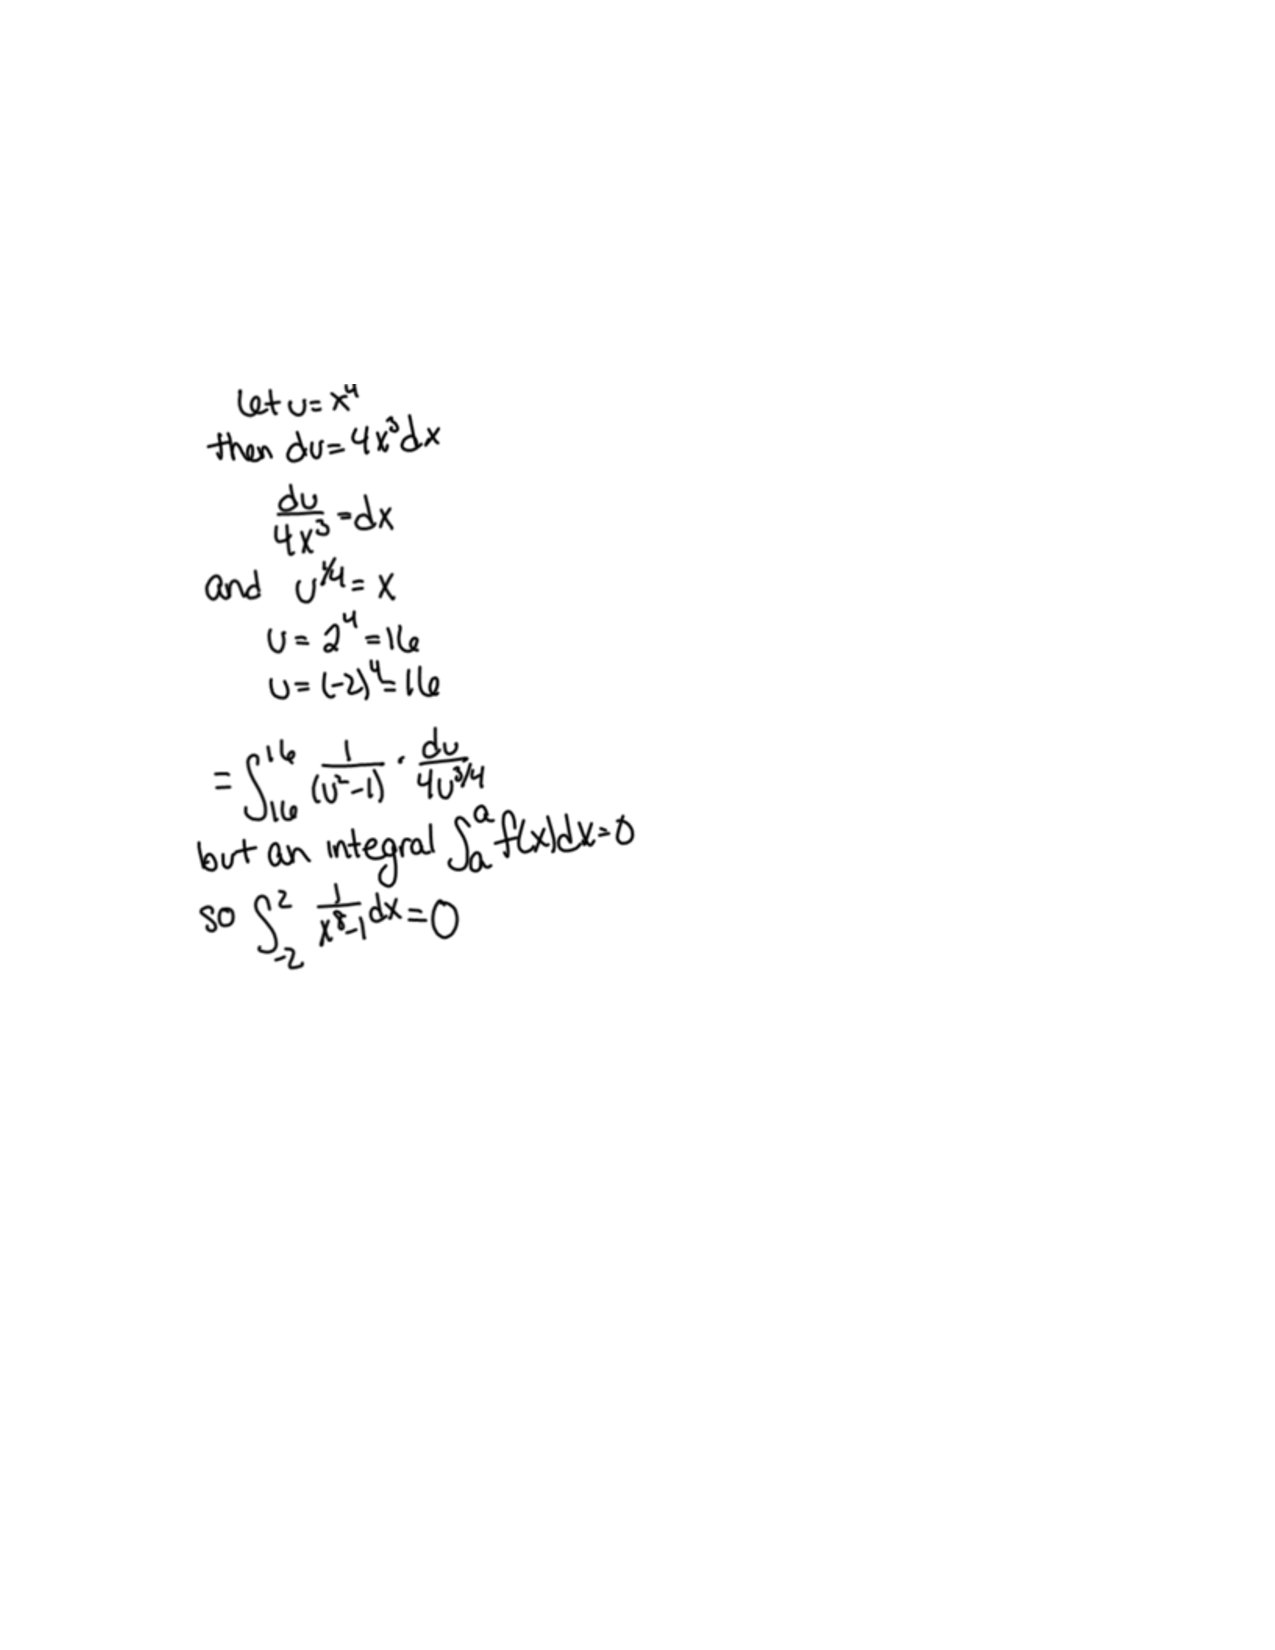
\includegraphics[trim= 170 420 250 180]{Figure1.pdf}
%\end{image}

%add a ``.'' below when used in a specific directory.
\newcommand{\RR}{\mathbb R}
\renewcommand{\d}{\,d}
\newcommand{\dd}[2][]{\frac{d #1}{d #2}}
\renewcommand{\l}{\ell}
\newcommand{\ddx}{\frac{d}{dx}}
\newcommand{\dfn}{\textbf}
\newcommand{\eval}[1]{\bigg[ #1 \bigg]}

\usepackage{multicol}

\renewenvironment{freeResponse}{
\ifhandout\setbox0\vbox\bgroup\else
\begin{trivlist}\item[\hskip \labelsep\bfseries Solution:\hspace{2ex}]
\fi}
{\ifhandout\egroup\else
\end{trivlist}
\fi} %% we can turn off input when making a master document


\title{Section 8.3: Separable Differential Equations}  

\begin{document}
\begin{abstract}		\end{abstract}
\maketitle




\section{Warm up:}
	Which of the following differential equations are separable?
	\begin{enumerate}
	\item $y' = \frac{ty}{t^2+1}$,
	\item $\frac{dy}{dx} =x^2 \sin (3y) -x^2$,
	\item $y' = t^2 - y$.
	\end{enumerate}

	\begin{freeResponse}
	\begin{enumerate}
	\item Yes, it is separable. $y' = y \cdot \frac{t}{t^2+1}$.
	\item Yes, it is separable. $\frac{dy}{dx} = x^2 \left( \sin(3y)-1 \right)$.
	\item No, it is not separable. $t^2-y$ can not be written in the form $F(t) \cdot G(y)$. 
	\end{enumerate}
	\end{freeResponse}
	
\begin{instructorNotes}

\end{instructorNotes}








\section{Group work:}



%problem 3
\begin{problem}
Find a specific solution to the differential equation $\dd[y]{x} = x^{-2} \arctan(x)$ if $y(1)=5$.
	\begin{freeResponse}
	First note that
		\[
		y = \int x^{-2} \arctan(x) \d x.
		\]
	To solve this integral, we use integration by parts with
		{\color{red}
		\[
		u = \arctan(x)  			\qquad 	\d v = x^{-2} \d x
		\]
		\[
		\d u = \frac{1}{1+x^2} \d x  \qquad 	v = -\frac{1}{x}.
		\]
		}
	So
		\begin{align*}
		\int x^{-2} \arctan(x) \d x
		&= - \frac{1}{x} \arctan(x) + \int \frac{1}{x(1+x^2)} \d x.
		\end{align*}
	To complete this new integral, we use partial fractions.
		{\color{red}
		\begin{align*}
		&\frac{1}{x(1+x^2)} = \frac{A}{x} + \frac{Bx+C}{1+x^2}  \\
		\Longrightarrow \qquad &1 = A(1+x^2) + (Bx+C)x  \\
		\Longrightarrow \qquad &1 = (A+B)x^2 + Cx + A.
		\end{align*}
	Comparing coefficients, we see that $A=1$, $C+0$, and $B = -1$.  
		}
		
	Thus
		\begin{align*}
		y &= \int x^{-2} \arctan(x) \d x  \\
		&= - \frac{1}{x} \arctan(x) + \int \frac{1}{x(1+x^2)} \d x  \\
		&= - \frac{1}{x} \arctan(x) + \int \left( \frac{1}{x} - \frac{x}{1+x^2} \right) \d x  \\
		&= - \frac{1}{x} \arctan(x) + \ln|x| - \frac{1}{2} \ln(1+x^2) + C.
		\end{align*}
	To finish, we use the initial condition to solve for $C$.
		\begin{align*}
		5 = y(1) &= - \frac{\pi}{4} + 0 - \frac{1}{2} \ln(2) + C  \\
		\Longrightarrow \qquad C &= 5 + \frac{\pi}{4} + \frac{1}{2} \ln(2).
		\end{align*}
	Therefore
		\[
		y(t) = - \frac{1}{x} \arctan(x) + \ln|x| - \frac{1}{2} \ln(1+x^2) + 5 + \frac{\pi}{4} + \frac{1}{2} \ln(2).
		\]
	\end{freeResponse}

\end{problem}

\begin{instructorNotes}
This is a straight forward antiderivative problem.  
The real interest here is finding the antiderivative using integration by parts and then partial fractions.  
\end{instructorNotes}








%problem 4
\begin{problem}
Find a specific solution to the initial value problem
	\[
	\dd[y]{x} = x^2 \sin(x), \qquad y(0) = 5.
	\]
	
	\begin{freeResponse}
	First, notice that
		\[
		y = \int x^2 \sin(x) \d x.
		\]
	To solve this integral, we use integration by parts twice.  
		{\color{red}
		\[
		u = x^2 		\qquad	\d v = \sin(x) \d x
		\]
		\[
		\d u = 2x \d x	\qquad	v = -\cos(x).
		\]
		}
	So
		\begin{align*}
		\int x^2 \sin(x) \d x
		&= -x^2 \cos(x) + \int 2x \cos (x) \d x.
		\end{align*}
	Now we use
		{\color{red}
		\[
		u = 2x 		\qquad	\d v = \cos(x) \d x
		\]
		\[
		\d u = 2 \d x	\qquad	v = \sin(x).
		\]
		}
	Then
		\begin{align*}
		y &= \int x^2 \sin(x) \d x  \\
		&= -x^2 \cos(x) + \int 2x \cos (x) \d x  \\
		&= -x^2 \cos(x) + 2x\sin(x) - \int 2\sin(x) \d x  \\
		&= -x^2\cos(x) + 2x\sin(x) + 2\cos(x) + C.
		\end{align*}
	Finally, to finish the problem, we solve for $C$.  
		\begin{align*}
		5 = y(0) &= 0 + 0 + 2 + C  \\
		\Longrightarrow \qquad C &= 3.
		\end{align*}
	Thus,
		\[
		y(t) = -x^2\cos(x) + 2x\sin(x) + 2\cos(x) + 3.
		\]
	\end{freeResponse}
	
\end{problem}



%Problem 5
\begin{problem}
Solve the following differential equations assuming that $y(4)=5$.
	\begin{enumerate}

	
	
	
	\item 	$y'=x+xy^2$
	\begin{freeResponse}
		\begin{align*}
		&y' = x+xy^2  \\
		\Longrightarrow 	\qquad	&\dd[y]{x} = x(1+y^2)  \\
		\Longrightarrow 	\qquad	&\frac{\d y}{1+y^2} = x \d x.
		\end{align*}
	So this equation \dfn{is} separable.
	To solve, we integrate both sides of the equation:
		\begin{align}
		&\int \frac{1}{1+y^2} \d y = \int x \d x  \nonumber \\
		\Longrightarrow 	\qquad	&\arctan(y) = \frac{1}{2} x^2 + C  \label{equation 1 for y}\\
		\Longrightarrow 	\qquad	&y = \tan \left( \frac{1}{2} x^2 + C \right).  \nonumber
		\end{align}
	To find $C$, we plug the initial condition $y(4) = 5$ into equation \eqref{equation 1 for y} and solve for $C$.
		\begin{align*}
		&\arctan(5) = \frac{1}{2} (4)^2 + C = 8 + C  \\
		\Longrightarrow 	\qquad	&C = \arctan(5) - 8.
		\end{align*}
	So
		\[
		y = \tan \left( \frac{1}{2} x^2 + \arctan(5) - 8 \right).
		\]
	\end{freeResponse}
	
	
	
	\item 	$y' = e^{2x-y}$
	\begin{freeResponse}
		\begin{align}
		&y' = e^{2x-y}  \nonumber \\
		\Longrightarrow 	\qquad	&\dd[y]{x} = \frac{e^{2x}}{e^y}  \nonumber \\
		\Longrightarrow 	\qquad	&e^y \d y = e^{2x} \d x  \label{eqn 2}
		\end{align}
	and so this \dfn{is} a separable equation.  
	To solve, we integrate both sides of equation \eqref{eqn 2}.
		\begin{align}
		&\int e^y \d y = \int e^{2x} \d x  \nonumber  \\
		\Longrightarrow 	\qquad	&e^y = \frac{1}{2} e^{2x} + C  \label{eqn 3}  \\
		\Longrightarrow 	\qquad	&y = \ln \left( \frac{1}{2} e^{2x} + C \right).  \nonumber
		\end{align}
	To find $C$, we plug into equation \eqref{eqn 3} and solve for $C$:
		\begin{align*}
		&e^5 = \frac{1}{2} e^8 + C  \\
		\Longrightarrow 	\qquad	&C = e^5 - \frac{1}{2} e^8.
		\end{align*}
	Therefore
		\[
		y = \ln \left( \frac{1}{2} e^{2x} + e^5 - \frac{1}{2}e^8 \right).
		\]
	\end{freeResponse}
	\end{enumerate}
	
\end{problem}

\begin{instructorNotes}
Part (b) is the only non-separable equation.  
Students may need help recognizing that they can divide by the entire right side of both sides.  
Also, some results may only define $y$ implicitly.
\end{instructorNotes}


	
	
	
	
	
	
	
	
	

	










								
				
				
	














\end{document} 


















